\chapter{Installation And Configuration
	\label{ch:Installation And Configuration}}

In this chapter installation and configuration of \textbf{Hyperledger Composer }will be shown with dummy coding data.
The installation is for Ubuntu although Mac installation is also available if you are interested in that you can follow it on their official documentation on this Link.

\section{Installation}
\subsection{Pre-Requisites}
Open terminal by Ctrl+T and run these command. These will not run and ask you to install curl. Simply install curl and run this command.Make sure not to use sudo to run these commands.
\begin{figure}[h]
	\centering
	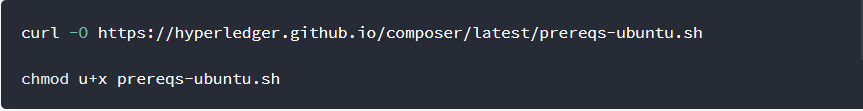
\includegraphics[width=450px]{figures/installation/1.png}
	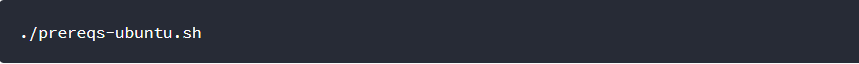
\includegraphics[width=450px]{figures/installation/2.png}
\end{figure}

The installation we have done above include textbf{Docker Node Git Python}
\subsection{Editor}
You can use whatever editor you want we recommend using \textbf{Visual Studio Code}.
\section{Installing Development Environment}
\subsection{Installing Command Line Tools}
\begin{figure}[h]
	\centering
	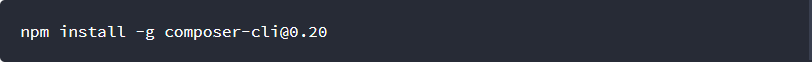
\includegraphics[width=450px]{figures/installation/3.png}
	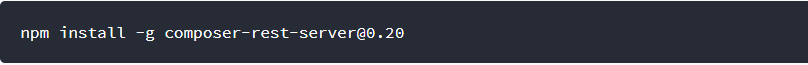
\includegraphics[width=450px]{figures/installation/4.png}
	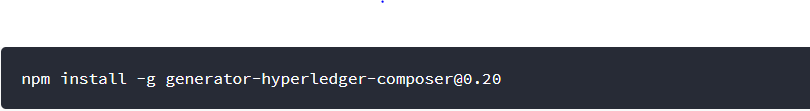
\includegraphics[width=450px]{figures/installation/5.png}
	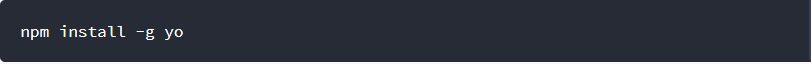
\includegraphics[width=450px]{figures/installation/6.png}
\end{figure}
\subsection{Installing Playground}
This is a playground tool for fabric in which you have to write the files (model, logic, permission, query)as discussed in the previous chapters 
\begin{figure}[h]
	\centering
	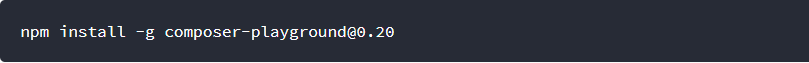
\includegraphics[width=450px]{figures/installation/7.png}
\end{figure}
\newpage
\subsection{Downloading Fabric}
\begin{figure}[h]
	\centering
	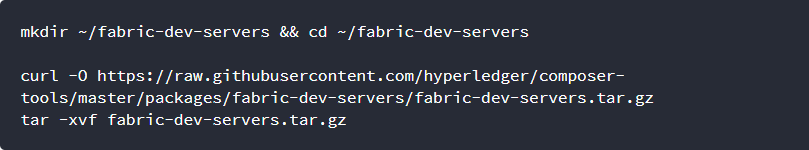
\includegraphics[width=450px]{figures/installation/8.png}
	\newline\newline
	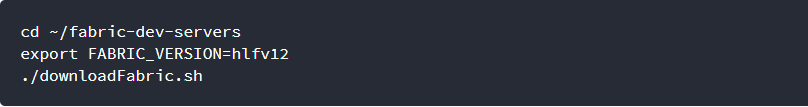
\includegraphics[width=450px]{figures/installation/9.png}

\end{figure}

Now the development installation is complete. \\To start fabric go to directory \textbf{fabric-dev-servers} and use this command.\\
\textbf{./startFabric.sh}
\\To stop fabric use this command inside the same directory.\\
\textbf{./stopFabric.sh}
\\And to open playground in the browser use any where in the terminal. \\
\textbf{composer-playground}
\\make sure not to use \textbf{sudo} with these commands.
\\Congratulations you have completed all installation now we will move on deployment.

\section{Deployment of Composer}
\begin{itemize}
	\item Open the composer playground and click on \textbf{Deploy a new business network}
	\item Name your business network 
	\item Select empty-business-network
	\item Now click on Deploy
\end{itemize}
Once the network is deployed connect to it. After connecting to network you have to add / write your files here.
\subsection{Adding Model File}
\begin{itemize}
	\item Click on \textbf{Model File} to view it, delete the code written there and add the following in there
\end{itemize}
\begin{figure}[h]
	\centering
	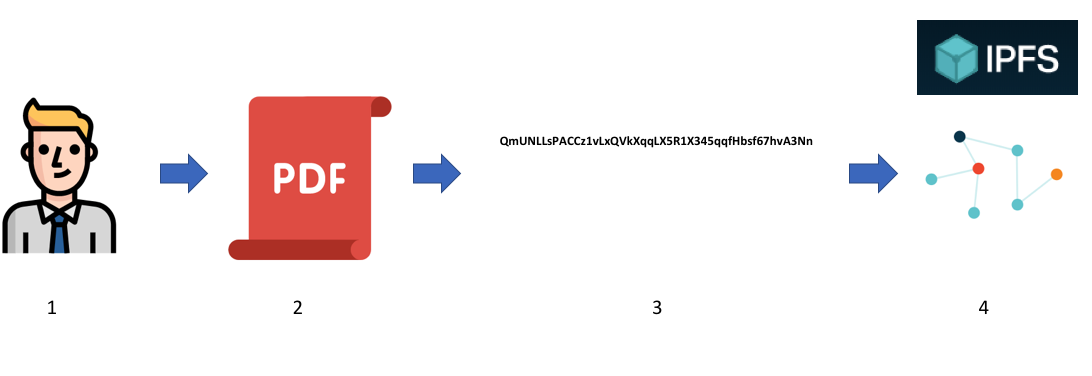
\includegraphics[width=450px]{figures/installation/10.png}
\end{figure}
\newpage
\subsection{Adding your Logic File}
\begin{itemize}
	\item Click on add file and choose script file
	\item Delete the code and add the following code
\end{itemize}

\begin{figure}[h]
	\centering
	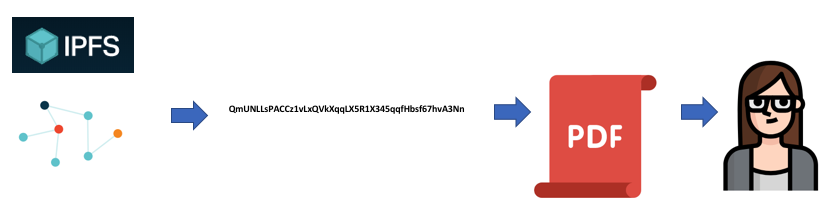
\includegraphics[width=450px]{figures/installation/11.png}
\end{figure}
This is enough for testing the deployment of fabric.
\section{Deployment of business network}
\subsection{Creating business network structure}
Run this command 
\begin{figure}[h]
	\centering
	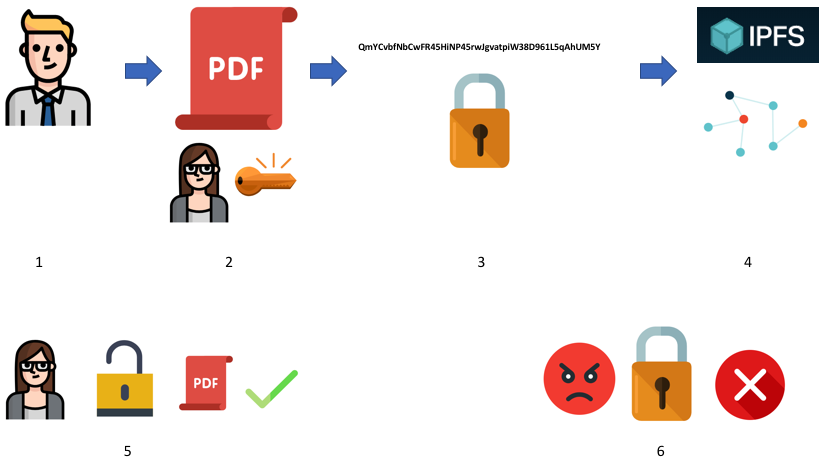
\includegraphics[width=450px]{figures/installation/12.png}
\end{figure}

\subsection{Generating business network archive}
Run this command 
\begin{figure}[h]
	\centering
	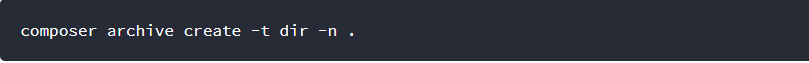
\includegraphics[width=450px]{figures/installation/13.png}
\end{figure}

\subsection{Installing business network}
Run this command 
\begin{figure}[h]
	\centering
	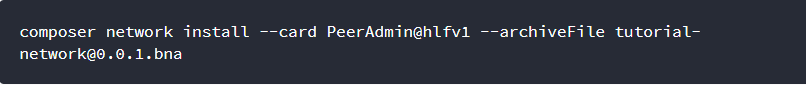
\includegraphics[width=450px]{figures/installation/14.png}
\end{figure}

\subsection{Starting business network}
Run this command 
\begin{figure}[h]
	\centering
	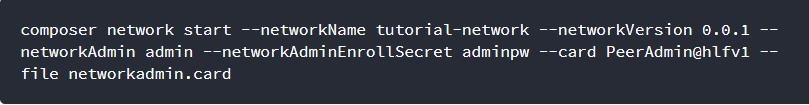
\includegraphics[width=450px]{figures/installation/15.png}
\end{figure}
\subsection{Importing network administrator card}
Run this command 
\begin{figure}[h]
	\centering
	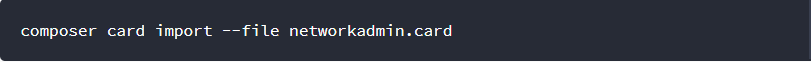
\includegraphics[width=450px]{figures/installation/16.png}
\end{figure}
\newpage
\section{Genrating rest server}

Run this command. 
\begin{figure}[h]
	\centering
	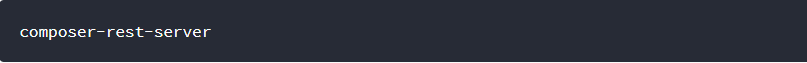
\includegraphics[width=450px]{figures/installation/18.png}
\end{figure}\\
You will be asked to give 
\begin{itemize}
	\item Network card name. 
	\item Select never use namespaces
	\item After that select textbf{No} to everything
\end{itemize}



